% Options for packages loaded elsewhere
\PassOptionsToPackage{unicode}{hyperref}
\PassOptionsToPackage{hyphens}{url}
\PassOptionsToPackage{dvipsnames,svgnames,x11names}{xcolor}
%
\documentclass[
]{interact}

\usepackage{amsmath,amssymb}
\usepackage{lmodern}
\usepackage{iftex}
\ifPDFTeX
  \usepackage[T1]{fontenc}
  \usepackage[utf8]{inputenc}
  \usepackage{textcomp} % provide euro and other symbols
\else % if luatex or xetex
  \usepackage{unicode-math}
  \defaultfontfeatures{Scale=MatchLowercase}
  \defaultfontfeatures[\rmfamily]{Ligatures=TeX,Scale=1}
\fi
% Use upquote if available, for straight quotes in verbatim environments
\IfFileExists{upquote.sty}{\usepackage{upquote}}{}
\IfFileExists{microtype.sty}{% use microtype if available
  \usepackage[]{microtype}
  \UseMicrotypeSet[protrusion]{basicmath} % disable protrusion for tt fonts
}{}
\makeatletter
\@ifundefined{KOMAClassName}{% if non-KOMA class
  \IfFileExists{parskip.sty}{%
    \usepackage{parskip}
  }{% else
    \setlength{\parindent}{0pt}
    \setlength{\parskip}{6pt plus 2pt minus 1pt}}
}{% if KOMA class
  \KOMAoptions{parskip=half}}
\makeatother
\usepackage{xcolor}
\setlength{\emergencystretch}{3em} % prevent overfull lines
\setcounter{secnumdepth}{5}
% Make \paragraph and \subparagraph free-standing
\ifx\paragraph\undefined\else
  \let\oldparagraph\paragraph
  \renewcommand{\paragraph}[1]{\oldparagraph{#1}\mbox{}}
\fi
\ifx\subparagraph\undefined\else
  \let\oldsubparagraph\subparagraph
  \renewcommand{\subparagraph}[1]{\oldsubparagraph{#1}\mbox{}}
\fi

\usepackage{color}
\usepackage{fancyvrb}
\newcommand{\VerbBar}{|}
\newcommand{\VERB}{\Verb[commandchars=\\\{\}]}
\DefineVerbatimEnvironment{Highlighting}{Verbatim}{commandchars=\\\{\}}
% Add ',fontsize=\small' for more characters per line
\usepackage{framed}
\definecolor{shadecolor}{RGB}{241,243,245}
\newenvironment{Shaded}{\begin{snugshade}}{\end{snugshade}}
\newcommand{\AlertTok}[1]{\textcolor[rgb]{0.68,0.00,0.00}{#1}}
\newcommand{\AnnotationTok}[1]{\textcolor[rgb]{0.37,0.37,0.37}{#1}}
\newcommand{\AttributeTok}[1]{\textcolor[rgb]{0.40,0.45,0.13}{#1}}
\newcommand{\BaseNTok}[1]{\textcolor[rgb]{0.68,0.00,0.00}{#1}}
\newcommand{\BuiltInTok}[1]{\textcolor[rgb]{0.00,0.23,0.31}{#1}}
\newcommand{\CharTok}[1]{\textcolor[rgb]{0.13,0.47,0.30}{#1}}
\newcommand{\CommentTok}[1]{\textcolor[rgb]{0.37,0.37,0.37}{#1}}
\newcommand{\CommentVarTok}[1]{\textcolor[rgb]{0.37,0.37,0.37}{\textit{#1}}}
\newcommand{\ConstantTok}[1]{\textcolor[rgb]{0.56,0.35,0.01}{#1}}
\newcommand{\ControlFlowTok}[1]{\textcolor[rgb]{0.00,0.23,0.31}{#1}}
\newcommand{\DataTypeTok}[1]{\textcolor[rgb]{0.68,0.00,0.00}{#1}}
\newcommand{\DecValTok}[1]{\textcolor[rgb]{0.68,0.00,0.00}{#1}}
\newcommand{\DocumentationTok}[1]{\textcolor[rgb]{0.37,0.37,0.37}{\textit{#1}}}
\newcommand{\ErrorTok}[1]{\textcolor[rgb]{0.68,0.00,0.00}{#1}}
\newcommand{\ExtensionTok}[1]{\textcolor[rgb]{0.00,0.23,0.31}{#1}}
\newcommand{\FloatTok}[1]{\textcolor[rgb]{0.68,0.00,0.00}{#1}}
\newcommand{\FunctionTok}[1]{\textcolor[rgb]{0.28,0.35,0.67}{#1}}
\newcommand{\ImportTok}[1]{\textcolor[rgb]{0.00,0.46,0.62}{#1}}
\newcommand{\InformationTok}[1]{\textcolor[rgb]{0.37,0.37,0.37}{#1}}
\newcommand{\KeywordTok}[1]{\textcolor[rgb]{0.00,0.23,0.31}{#1}}
\newcommand{\NormalTok}[1]{\textcolor[rgb]{0.00,0.23,0.31}{#1}}
\newcommand{\OperatorTok}[1]{\textcolor[rgb]{0.37,0.37,0.37}{#1}}
\newcommand{\OtherTok}[1]{\textcolor[rgb]{0.00,0.23,0.31}{#1}}
\newcommand{\PreprocessorTok}[1]{\textcolor[rgb]{0.68,0.00,0.00}{#1}}
\newcommand{\RegionMarkerTok}[1]{\textcolor[rgb]{0.00,0.23,0.31}{#1}}
\newcommand{\SpecialCharTok}[1]{\textcolor[rgb]{0.37,0.37,0.37}{#1}}
\newcommand{\SpecialStringTok}[1]{\textcolor[rgb]{0.13,0.47,0.30}{#1}}
\newcommand{\StringTok}[1]{\textcolor[rgb]{0.13,0.47,0.30}{#1}}
\newcommand{\VariableTok}[1]{\textcolor[rgb]{0.07,0.07,0.07}{#1}}
\newcommand{\VerbatimStringTok}[1]{\textcolor[rgb]{0.13,0.47,0.30}{#1}}
\newcommand{\WarningTok}[1]{\textcolor[rgb]{0.37,0.37,0.37}{\textit{#1}}}

\providecommand{\tightlist}{%
  \setlength{\itemsep}{0pt}\setlength{\parskip}{0pt}}\usepackage{longtable,booktabs,array}
\usepackage{calc} % for calculating minipage widths
% Correct order of tables after \paragraph or \subparagraph
\usepackage{etoolbox}
\makeatletter
\patchcmd\longtable{\par}{\if@noskipsec\mbox{}\fi\par}{}{}
\makeatother
% Allow footnotes in longtable head/foot
\IfFileExists{footnotehyper.sty}{\usepackage{footnotehyper}}{\usepackage{footnote}}
\makesavenoteenv{longtable}
\usepackage{graphicx}
\makeatletter
\def\maxwidth{\ifdim\Gin@nat@width>\linewidth\linewidth\else\Gin@nat@width\fi}
\def\maxheight{\ifdim\Gin@nat@height>\textheight\textheight\else\Gin@nat@height\fi}
\makeatother
% Scale images if necessary, so that they will not overflow the page
% margins by default, and it is still possible to overwrite the defaults
% using explicit options in \includegraphics[width, height, ...]{}
\setkeys{Gin}{width=\maxwidth,height=\maxheight,keepaspectratio}
% Set default figure placement to htbp
\makeatletter
\def\fps@figure{htbp}
\makeatother
\newlength{\cslhangindent}
\setlength{\cslhangindent}{1.5em}
\newlength{\csllabelwidth}
\setlength{\csllabelwidth}{3em}
\newlength{\cslentryspacingunit} % times entry-spacing
\setlength{\cslentryspacingunit}{\parskip}
\newenvironment{CSLReferences}[2] % #1 hanging-ident, #2 entry spacing
 {% don't indent paragraphs
  \setlength{\parindent}{0pt}
  % turn on hanging indent if param 1 is 1
  \ifodd #1
  \let\oldpar\par
  \def\par{\hangindent=\cslhangindent\oldpar}
  \fi
  % set entry spacing
  \setlength{\parskip}{#2\cslentryspacingunit}
 }%
 {}
\usepackage{calc}
\newcommand{\CSLBlock}[1]{#1\hfill\break}
\newcommand{\CSLLeftMargin}[1]{\parbox[t]{\csllabelwidth}{#1}}
\newcommand{\CSLRightInline}[1]{\parbox[t]{\linewidth - \csllabelwidth}{#1}\break}
\newcommand{\CSLIndent}[1]{\hspace{\cslhangindent}#1}

\usepackage{orcidlink}
\makeatletter
\makeatother
\makeatletter
\makeatother
\makeatletter
\@ifpackageloaded{caption}{}{\usepackage{caption}}
\AtBeginDocument{%
\ifdefined\contentsname
  \renewcommand*\contentsname{Table of contents}
\else
  \newcommand\contentsname{Table of contents}
\fi
\ifdefined\listfigurename
  \renewcommand*\listfigurename{List of Figures}
\else
  \newcommand\listfigurename{List of Figures}
\fi
\ifdefined\listtablename
  \renewcommand*\listtablename{List of Tables}
\else
  \newcommand\listtablename{List of Tables}
\fi
\ifdefined\figurename
  \renewcommand*\figurename{Figure}
\else
  \newcommand\figurename{Figure}
\fi
\ifdefined\tablename
  \renewcommand*\tablename{Table}
\else
  \newcommand\tablename{Table}
\fi
}
\@ifpackageloaded{float}{}{\usepackage{float}}
\floatstyle{ruled}
\@ifundefined{c@chapter}{\newfloat{codelisting}{h}{lop}}{\newfloat{codelisting}{h}{lop}[chapter]}
\floatname{codelisting}{Listing}
\newcommand*\listoflistings{\listof{codelisting}{List of Listings}}
\makeatother
\makeatletter
\@ifpackageloaded{caption}{}{\usepackage{caption}}
\@ifpackageloaded{subcaption}{}{\usepackage{subcaption}}
\makeatother
\makeatletter
\@ifpackageloaded{tcolorbox}{}{\usepackage[many]{tcolorbox}}
\makeatother
\makeatletter
\@ifundefined{shadecolor}{\definecolor{shadecolor}{rgb}{.97, .97, .97}}
\makeatother
\makeatletter
\makeatother
\ifLuaTeX
  \usepackage{selnolig}  % disable illegal ligatures
\fi
\IfFileExists{bookmark.sty}{\usepackage{bookmark}}{\usepackage{hyperref}}
\IfFileExists{xurl.sty}{\usepackage{xurl}}{} % add URL line breaks if available
\urlstyle{same} % disable monospaced font for URLs
\hypersetup{
  pdftitle={Demo arXiv template},
  pdfauthor={H. Sherry Zhang; Collaborators},
  pdfkeywords={indexes, data pipeline, software design},
  colorlinks=true,
  linkcolor={blue},
  filecolor={Maroon},
  citecolor={Blue},
  urlcolor={Blue},
  pdfcreator={LaTeX via pandoc}}

\title{Demo arXiv template}
\author{H. Sherry
Zhang$\textsuperscript{1}$~\orcidlink{0000-0002-7122-1463}, Collaborators$\textsuperscript{1}$}

\thanks{CONTACT: H. Sherry
Zhang. Email: \href{mailto:huize.zhang@monash.edu}{\nolinkurl{huize.zhang@monash.edu}}. }
\begin{document}
\captionsetup{labelsep=space}
\maketitle
\textsuperscript{1} Department of Econometrics and Business
Statistics, Monash University, Melbourne, VIC, Australia
\begin{abstract}
\begin{itemize}
\tightlist
\item
  indexes, useful, quantify severity, early monitoring,
\item
  A huge number of indexes have been proposed by domain experts,
  however, a large majority of them are not being adopted, reused, and
  compared in research or in practice.
\item
  One of the reasons for this is the plenty of indexes are quite complex
  and there is no obvious easy-to-use implementation to apply them to
  user's data.
\item
  The paper describes a general pipeline framework to construct indexes
  from spatio-temporal data,
\item
  This allows all the indexes to be constructed through a uniform data
  pipeline and different indexes to vary on the details of each step in
  the data pipeline and their orders.
\item
  The pipeline proposed aim to smooth the workflow of index construction
  through breaking down the complicated steps proposed by various
  indexes into small building blocks shared by most of the indexes.
\item
  The framework will be demonstrated with drought indexes as examples,
  but appliable in general to environmental indexes constructed from
  multivariate spatio-temporal data
\end{itemize}
\end{abstract}
\begin{keywords}
\def\sep{;\ }
indexes\sep data pipeline\sep 
software design
\end{keywords}
\ifdefined\Shaded\renewenvironment{Shaded}{\begin{tcolorbox}[interior hidden, boxrule=0pt, enhanced, borderline west={3pt}{0pt}{shadecolor}, sharp corners, breakable, frame hidden]}{\end{tcolorbox}}\fi

\hypertarget{introduction}{%
\section{Introduction}\label{introduction}}

\textbf{Why index is useful, why people care about indexes}

\emph{incorporate the following in why using index: multiple pieces of
information (variables) that need to be taken into account}

Many concepts relevant to decision making cannot be directly measured,
however, they are crucial for resource allocation, early prevention, and
other operational purpose.

\begin{itemize}
\tightlist
\item
  USDM and European Drought Observatory publishes drought indicator to
  {[}\ldots{]},
\item
  NOAA and BOM producing forecast on El Nino alert system to
  {[}\ldots{]}
\item
  OECD and UN producing indexes measuring socio-economic aspects of
  country for policy making.
\end{itemize}

There decision making often needs to consider multiple aspects and
indexes is a statistical tool to pack these information into a single
number, making it easier for policy makers and public communication.

\textbf{Define what is an index, what is not}

\begin{itemize}
\tightlist
\item
  Indexes can be composed from single variables or multiple variables
  (composite index)
\item
  to make the definition even more complex is that indexes themselves
  are used with other variables to compose indexes (many drought indexes
  using an index called SPI).
\item
  Some indexes may be more simple than you think:

  \begin{itemize}
  \tightlist
  \item
    a single transformation (NDVI (Tucker 1979) takes two spectrum: red
    and near-infrared and calculates as
    \((\text{NIR} + \text{Red})/(\text{NIR} + \text{Red})\))
  \item
    indexes sometimes are similar to features extracted from time series
    data: ETCCDI climate change indices (Zhang 2020): SU - number of
    summer days: annual count of days when TX \textgreater{} 25 degree
  \end{itemize}
\item
  The index pipeline and software implementation we propose are
  applicable to all indexes mentioned above, while the main focus of
  this paper is on indexes that combine multiple variables/indexes since
  more skills are required to diagnose those indexes to understand how
  they behave.
\end{itemize}

\textbf{What is the challenges with current index construction}

\begin{itemize}
\tightlist
\item
  Difficult to reach consensus on composite/multivariate indexes.
\item
  Given the complexity of multivariate indexes as compared to univariate
  indexes, it raises more doubt to persuade people to use it.
\item
  Typical ways to evaluate new indexes is to compare it with the
  standard indexes (i.e.~SPI in drought index) or a response variable
  (i.e.~crop yield for monitoring agricultural drought).
\item
  However, more doubt can still raises: Whether the variable used to
  construct the index is a good set of variables.
\item
  Does the index series capture the variables measures. Whether other
  ways of combining the variables results in difference in the index.
\item
  Being able to answer these questions help to prove the robustness,
  extendibility and dimensionality of the index, as proposed by xxx as
  criteria for (selecting?) indexes.
\end{itemize}

\textbf{what can be done if people adopt this pipeline/ why it is
beneficial?}

\begin{itemize}
\tightlist
\item
  In order to evaluate indexes, indexes need to be broken down into
  pieces that it constitutes and then we can analyse how each component
  will affect the index.
\item
  The OECD handbook (OECD, European Union, and Joint Research Centre -
  European Commission 2008) provides technical guidelines to construct
  composite indexes for comparing country performance for policy-making.
  This paper identifies a more general pipeline framework where
  statistical indexes (of all kinds) can be built from. Based on the
  pipeline, an R package is built to validate the indexes, {[}more
  details on the functionality here{]} from understanding multivariate
  relationships to uncertainty analysis.
\end{itemize}

\textbf{who would benefit from this paper}

\begin{itemize}
\tightlist
\item
  This work provides researchers actively developing new indexes with
  tools to evaluate the proposed indexes.
\item
  Helping index analysts to identify weakness in existing indexes for
  methodology improvement.
\end{itemize}

The rest of the paper is structured as follows:
Section~\ref{sec-pipeline} reviews the concept of data pipeline in R.
The pipeline framework for index construction is presented in
Section~\ref{sec-index-pipeline}. Section~\ref{sec-dev} explains how to
include a new building block in each pipeline module. Examples are given
in Section~\ref{sec-examples} to demonstrate the index construction with
the pipeline built.

\hypertarget{sec-pipeline}{%
\section{Data pipeline}\label{sec-pipeline}}

\emph{Think about if there is another word for data pipeline}

\textbf{Why you should care about pipeline}

Data pipeline is not a new concept to computing. It refers to a set of
data processing elements connected in series, where the output of one
element is the input of the next one. Wickham et al. (2009) argues that
whether made explicit or not, the pipeline has to be presented in every
graphics program. The paper also argues that breaking down graphic
rendering into steps is beneficial for understanding the implementation
and comparing between different graphic systems. The discussion on
pipeline construction is well documented in early interactive graphics
software: Buja et al. (1988), Sutherland et al. (2000), and Xie,
Hofmann, and Cheng (2014) and their pipeline steps include non-linear
transformation, variable standardization, randomization and dimension
reduction.

\textbf{What is pipeline, its underlying software design philosophy, and
how these are reflected in R}

One of the most commonly known pipeline examples is perhaps the Unix
pipeline where programs can be concatenated with \texttt{\textbar{}} to
flow the output from the last program into the next program, i.e.~

\begin{verbatim}
command 1 | command 2 | command 3 | ...
\end{verbatim}

To solve a complex problem, the Unix system builds simple programs that
do one thing well and work well together. This design is also reflected
in the tidyverse ecosystem in R. To solve a complicated data problem
using tidyverse, analysts typically build the solution using a
collection of tools from the tidyverse toolbox. The data object can flow
smoothly from one command to the next, safeguarded by the tidy data
format (Wickham 2014), which prescribes three rules on how to lay out
tabular data. The tidyverse tools also embrace a strong human-centered
design where function names are intuitive and easy to reference through
autocomplete. With the tidyverse design principle in mind, the tidymodel
suite enables analysts to build machine learning models through the data
pipeline. It includes typical tasks required in machine learning like
data resampling, feature engineering, model fitting, model tuning, and
model evaluation. An advantage of tidymodel pipeline over separate
software for individual models is that analysts no longer need to write
model-specific syntax to work with each model, but pipeline-specific
syntax that is applicable to all the models implemented in tidymodel.
This allows users to easily experiment with a collection of machine
learning models.

\textbf{Constructing indexes would also benefit from pipeline and
embracing the aforementioned design philosophy.}

In index construction, data pipeline is often presented in a workflow
diagram in the research paper to illustrate how the raw data is
transformed into the final indexes. This agrees with Wickham's argument
on the presence of the data pipeline, however, more often than not, the
pipeline is not made explicit in the software. Often the time, all the
steps are lumped into a single wrapper function, rather than being split
into smaller, modulated functions. This increases the cost of
maintaining and understanding the code base, gives analysts little
freedom to customise the indexes for specific needs, and hinders reusing
existing code for building new indexes. A pipeline approach unites a
range of indexes under a single data pipeline and analysts can compose
indexes from pipeline steps like building Legos from individual bricks.
In this workflow, analysts are not limited by indexes that have been
already proposed and can easily combine pipeline steps to compose novel
indexes. Analysis of the indexes (i.e.~calculation of uncertainty) is
also feasible by adding external code into the pipeline.

\hypertarget{sec-index-pipeline}{%
\section{A pipeline for building statistical
indexes}\label{sec-index-pipeline}}

\hypertarget{sec-toy-example}{%
\subsection{How does the pipeline constructin of an index look
like?}\label{sec-toy-example}}

Consider a commonly used drought index: Standardized
Precipitation-Evapotranspiration Index (SPEI) (Vicente-Serrano,
Beguería, and López-Moreno 2010). Its construction involves:

\begin{enumerate}
\def\labelenumi{\arabic{enumi})}
\tightlist
\item
  transform the average temperature (\texttt{TMED}) into potential
  evapotranspiration (\texttt{pet})
\item
  combine precipitation (\texttt{prcp}) and potential evapotranspiration
  (\texttt{pet}) into a single variable \texttt{diff}
\item
  aggregate the difference series with a sliding window
  (\texttt{.scale})
\item
  fit a distribution to the aggregated series, and
\item
  derive the index value from the normal density values.
\end{enumerate}

Conventionally approach may combine all these steps into a single
function, with some level of modularity. However, these modules may only
work for the selected index offered by the package.

Under the pipeline approach, analysts first need to identify which
module each step belongs to.

Below shows the pseudocode for constructing SPEI with the pipeline:

\begin{verbatim}
DATA %>% 
  var_trans(.method = thornthwaite, Tave = TMED, ..., .new_name = "pet") %>%
  dim_red(diff = prcp - pet) %>%
  aggregate(.var = diff, .scale = 12, .new_name = "agg") %>%
  dist_fit(.method = "lmoms", .var = agg, .dist = DIST) %>%
  augment(.var = agg)
\end{verbatim}

The pipeline construct allows for multiple \texttt{.scales} and
\texttt{.dist} to be evaluated in \texttt{aggregate()} and
\texttt{dist\_fit()} to compare index under different parameterisations.
The result can then be passed into the \texttt{ggplot2} to crease
visualisation. \textbf{?@fig-toy-example} compares the SPEI calculated
with two distributions (log-logistic and pearson III).

Apart from evaluating multiples parameters, the pipeline approach allows
the the steps written for one index can be directly extrapolate to
another index building within the pipeline. The flexibility of the
pipeline also integrate well with other existing packages, for examples,
fitting distributions using L-moment is commonly used when constructing
drought indexes. The package \texttt{lmomco} provides general L-moment
fits to a wide range of distributions and users can easily access to all
the distributions within the pipeline.

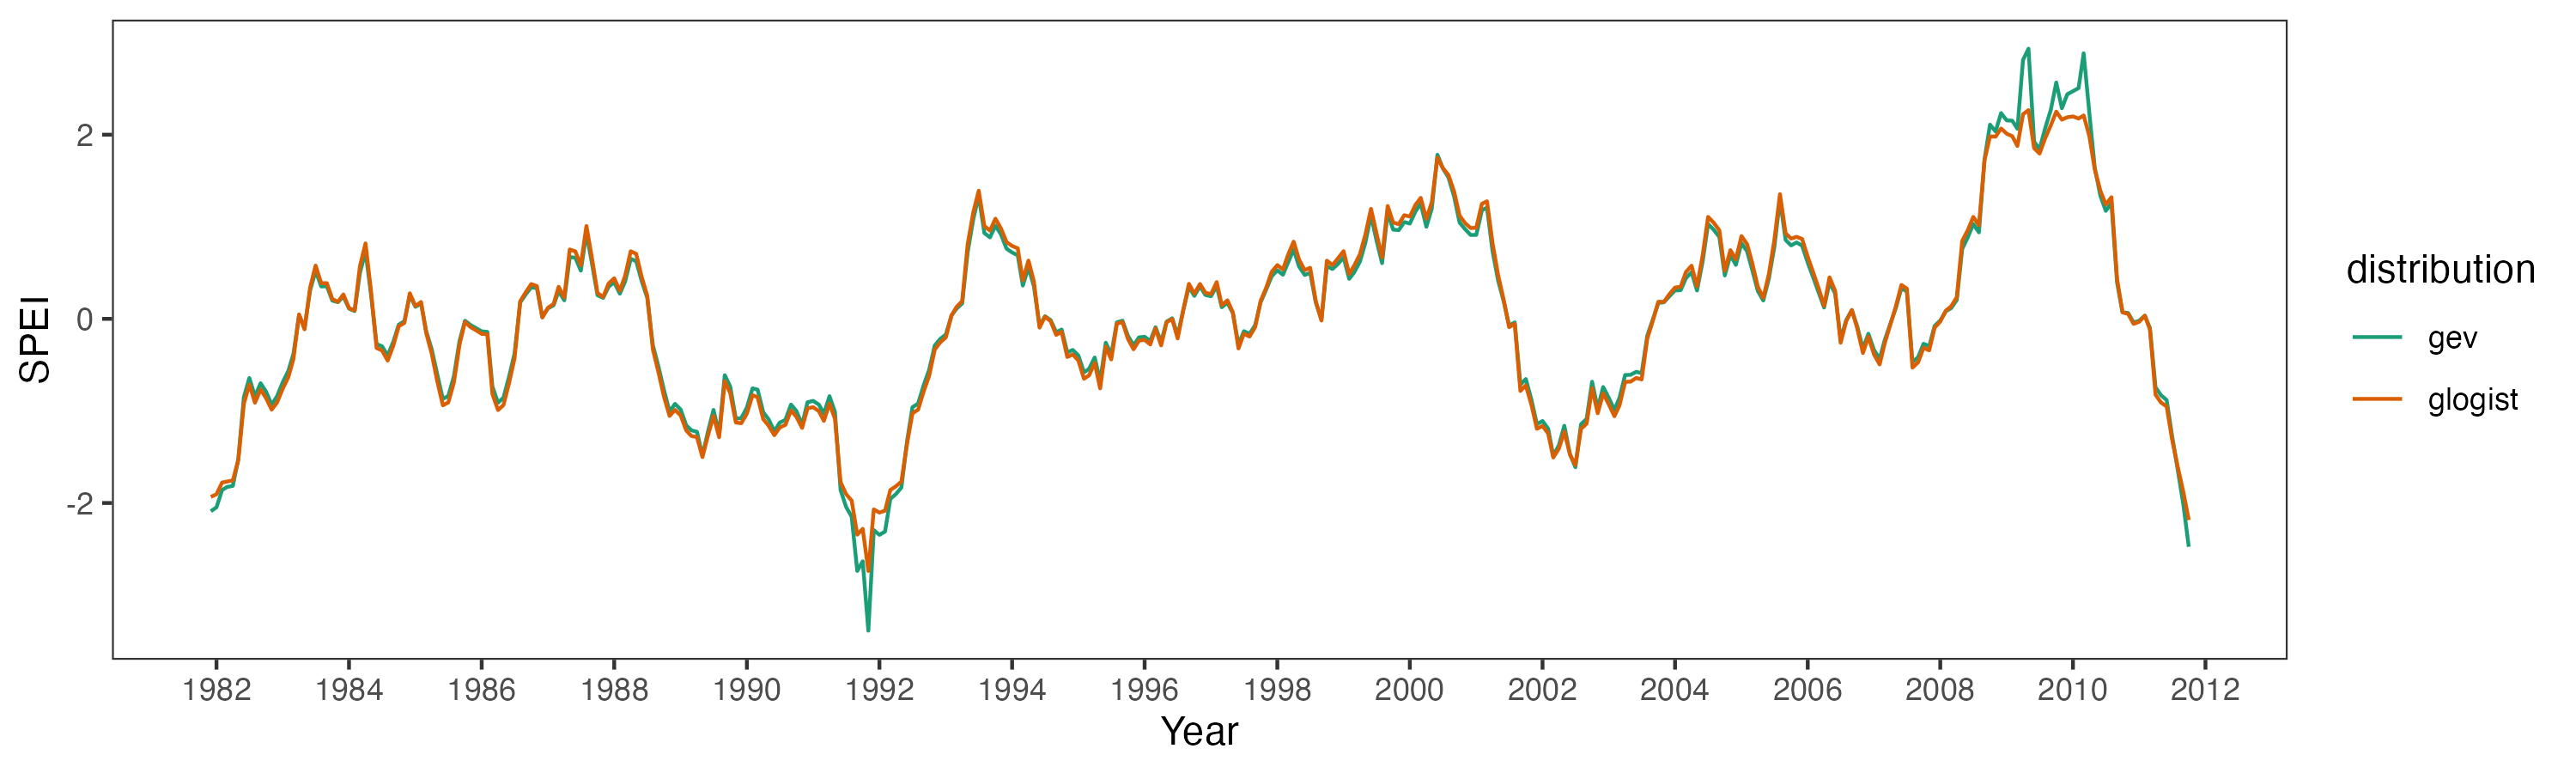
\includegraphics[width=10in,height=\textheight]{figures/toy-example-spei.png}

\hypertarget{pipeline-steps-for-constructing-indies}{%
\subsection{Pipeline steps for constructing
indies}\label{pipeline-steps-for-constructing-indies}}

\emph{any index can be broken down into multiple steps and then we can
do things with it: swap, change parameter, etc}

\emph{variables == indicators}

An overview of the pipeline is given in Figure~\ref{fig-pipeline-steps}
to illustrate the construction from raw data to the final indexes. The
pipeline includes eight modules for operations in the spatial, temporal,
and multivariate aspects of the data as well as modules for comparing
and communicating indexes. Analysts are free to select the modules they
need and arrange them in the order they see fit to construct indexes.
While the starting point of the pipeline is raw data, there are steps
prior to this that are crucial to the success of an index. For example,
the defined index needs to be useful for measuring the concept of
interest and variables need to be collected from reliable sources with
proper quality control.

Before elaborating each of the eight pipeline modules as subsections,
the data notation will be first introduced. Let
\(\mathbf{x}(\mathbf{s};\mathbf{t})\) denote the raw data with spatial,
temporal, and multivariate aspects: the spatial dimension
\(\mathbf{s} = (s_1, s_2, \cdots, s_n)^\prime\) is defined in the 2D
space: \(\mathbf{s} \in \mathcal{D}_s \subseteq \mathbb{R}^2\), the
temporal dimension \(\mathbf{t} = (t_1, t_2, \cdots, t_J)^\prime\) is
defined in the 1D space:
\(\mathbf{t} \in \mathcal{D}_t \subseteq \mathbb{R}\). When more than
one variable is involved, the multivariate data can also be written as:
\(\mathbf{x}(\mathbf{s}; \mathbf{t}) = (x_1(\mathbf{s}; \mathbf{t}), x_2(\mathbf{s}; \mathbf{t}), \cdots, x_P(\mathbf{s}; \mathbf{t}))^\prime\).

\begin{figure}

{\centering 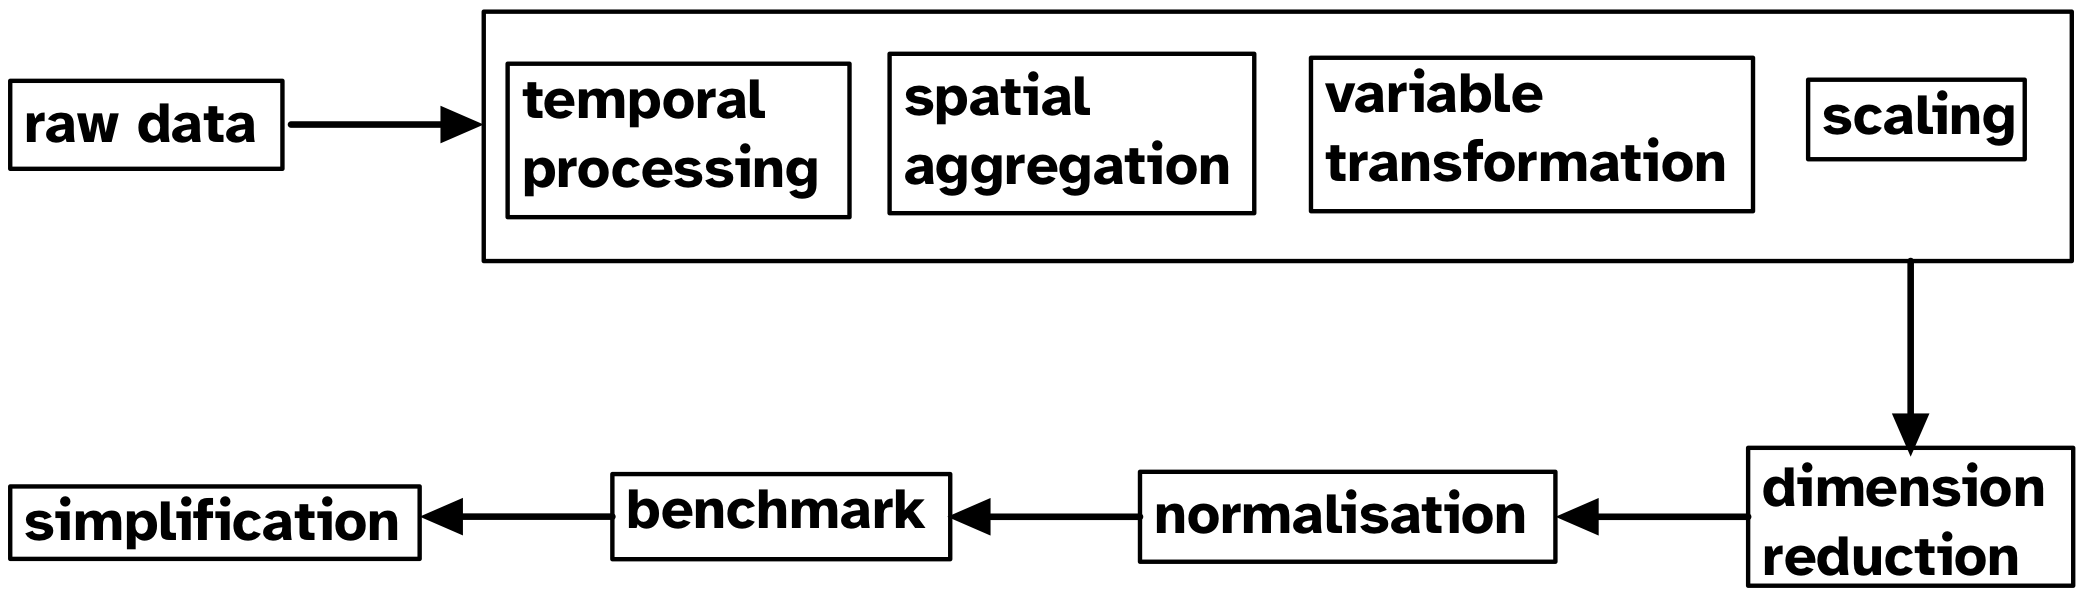
\includegraphics[width=1\textwidth,height=0.9\textheight]{figures/pipeline-steps.png}

}

\caption{\label{fig-pipeline-steps}Diagram of pipeline steps for index
construction. will need to be updated with better design and the
distribution fitting step.}

\end{figure}

\hypertarget{temporal-processing}{%
\subsubsection{Temporal processing}\label{temporal-processing}}

The construction of an index sometimes needs to consider information
from neighbouring time periods. The temporal processing is a general
operator on the time dimension of the data in the form of

\begin{equation}
f_{\mathcal{\psi}}(x(\mathbf{s};\mathbf{t})),
\end{equation}

where \(\psi \in \Psi \subseteq \mathbb{R}^{d_{\psi}}\) is the
parameters associated with the temporal operation and \(d_{\psi}\) is
the number of parameter of \(\psi\). A typical example of temporal
processing is aggregation, which is used in the drought index SPI to
measure the lack of precipitation for meteorological drought. In SPI,
monthly precipitation is aggregated by a time scale parameter \(k\):
\(x(s_i;t_{j^\prime}) = \sum_{j = j^\prime-k+1}^{j^\prime}x(s_i; t_j),\)
where \(j^\prime\) is the new time index after the aggregation. In this
notation, each spatial location is separately aggregated and
precipitation is summed from \(k\) month back, \(j^\prime - k + 1\), to
the current period, \(j^\prime\), to create the aggregated series,
indexed by \(j^\prime\).

\emph{more explicit on k will influence 1) long term vs.~short term, 2)
uncertainty}

The choice of time scales parameter \(k\) can result in variation in the
calculated index values: a small \(k\) of 3 or 6 months produces the
index more sensitive to individual months, while a large \(k\) of 24 or
36, an equivalent to a 2- or 3-year aggregation, gives dryness
information relative to the long term condition. As will be shown in
section {[}SECTION EXAMPLE{]}, this variation may even lead to
conflicting conclusions on the dry/wet condition of the area,
highlighting the importance to account for index uncertainty when
interpreting index values for decision-making.

\emph{Effective drought index}

\hypertarget{spatial-processing}{%
\subsubsection{Spatial processing}\label{spatial-processing}}

Spatial processing may be needed when indexes are not calculated
independently on each collected location or when variables collected
from multiple sources need to be fused before further processing. The
process can be written as a general operation in the form of

\begin{equation}
x(\mathbf{s}^\prime;\mathbf{t}) = g_{\mathcal{\theta}}(x(\mathbf{s};\mathbf{t})),
\end{equation}

where \(\theta \in \Theta \subseteq \mathbb{R}^{d_{\theta}}\) is the
associated parameters in the process and \(d_{\theta}\) is the number of
parameter of \(\theta\). An example of spatial processing is to align
variables collected in different resolutions. When variables are
collected at different resolutions, analysts may choose to down-sample
those in a finer resolution, \(i\), to match those in a coarser
resolution, \(i^\prime\). This is a spatial aggregation and if aggregate
using the mean, it can be written as

\begin{equation}
g(x) = \frac{\sum_{i \in i^\prime}x}{n_{i^\prime}},
\end{equation}

where \(i \in i^\prime\) includes all the cells from the finer
resolution in the coarser grid and \(n_{i^\prime}\) is the number of
observations falls into the coarser grid. Other examples of spatial
processing include 1) borrowing information from neighbouring spatial
locations to interpolate unobserved locations and 2) fusing variables
from ground measures with satellite imageries.

\hypertarget{variable-transformation}{%
\subsubsection{Variable transformation}\label{variable-transformation}}

The purpose of variable transformation is to create variables that fits
assumptions for further computing. These assumptions include a stable
variance, normal distribution, or a certain scale required by some
algorithms down the pipeline. Variable transformation is a general
notion of a functional transformation on the variable:

\begin{equation}
h_{\tau}(x(\mathbf{s};\mathbf{t})),
\end{equation}

where \(\tau \in T \subseteq \mathbb{R}^{d_{\tau}}\) is the parameter in
the transformation if any, and \(d_{\tau}\) is the number of parameter
of \(\tau\). Transformation is needed for data that are highly skewed
and some common transformations include log, quadratic, and square root
transformation.

\hypertarget{scaling}{%
\subsubsection{Scaling}\label{scaling}}

While scaling can be seen as a specific type of variable transformation,
it is separated into its own step to make the step explicit in the
pipeline. The key difference between the two steps is that variable
transformation typically changes the shape of the data while scaling
only changes the data scale and can usually be written in the form of

\begin{equation}
[x(s_i;t_j) - \alpha]/\gamma.
\end{equation}

For example, a z-score standardisation can be written in the above form
with \(\alpha = \bar{x}(s; t)\) and \(\gamma = \sigma(s; t)\), a min-max
standardisation uses \(\alpha = \min[x(s_i, t_j)]\) and
\(\gamma = \max[x(s_i, t_j)] - \min[x(s_i, t_j)]\).
Figure~\ref{fig-scale-var-trans-compare} shows a collection of variable
pre-processing operations and uses color to differentiate whether the
operation is a variable transformation or a scaling step. While both
variable transformation and scaling are pre-processing steps, the
scaling operations in green show the same distribution as the original
data.

\begin{figure}

{\centering 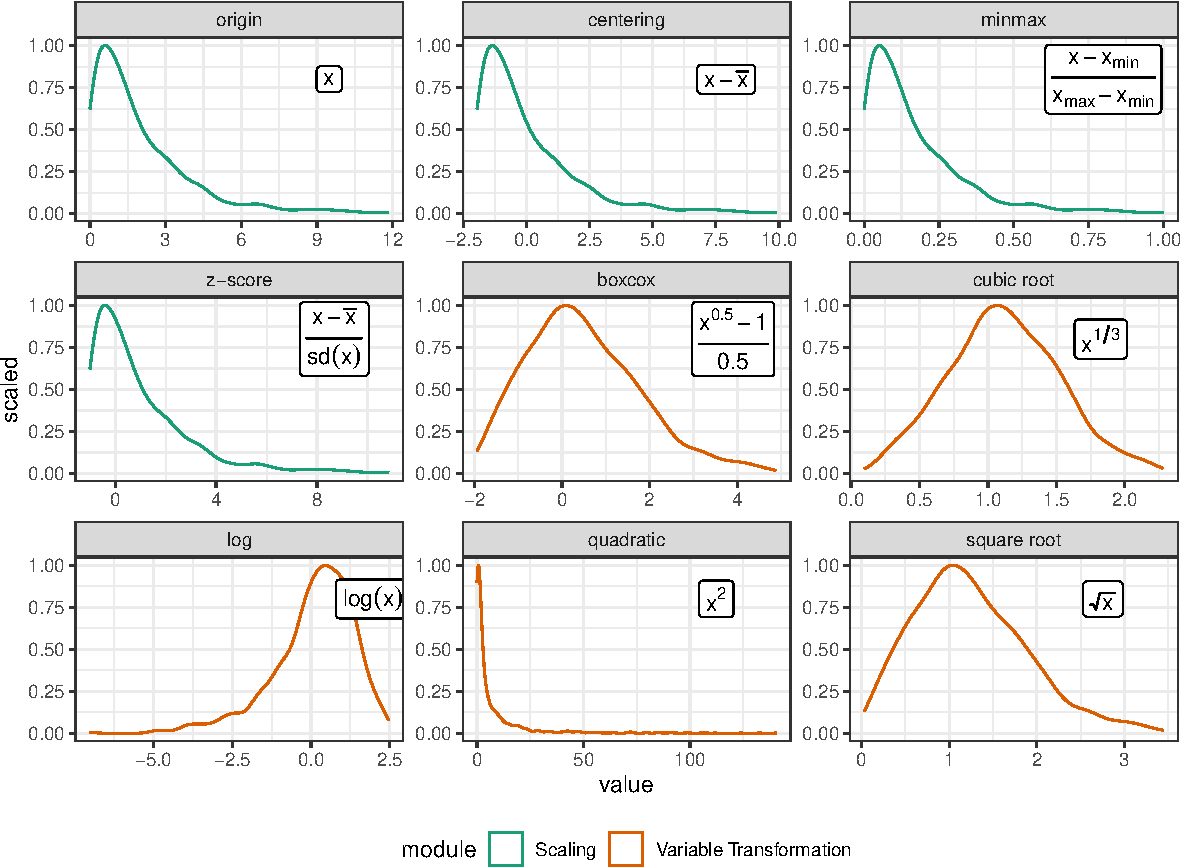
\includegraphics{tidyindex_files/figure-pdf/fig-scale-var-trans-compare-1.pdf}

}

\caption{\label{fig-scale-var-trans-compare}Comparison of operations in
scaling (green) and variable transformation (orange) steps in free
scale. Variables after the scaling operations have the same distribution
as the origin, while the distribution changes after variable
transformation.}

\end{figure}

\newpage

\hypertarget{dimension-reduction}{%
\subsubsection{Dimension reduction}\label{dimension-reduction}}

When indexes are constructed from multivariate information, dimension
reduction methods combine that information into a univariate series. In
the pipeline, dimension reduction includes methods that take
multivariate inputs and output the data in a lower dimension (often
univariate):

\begin{equation}
x_{p^*}(\mathbf{s}; \mathbf{t}) \rightarrow x_p(\mathbf{s}; \mathbf{t}),
\end{equation}

where \(p^* = 1, 2, \cdots, P^*\) and \(p = 1, 2, \cdots, P\) reduce the
variable dimension from \(P\) to \(P^*\). The most commonly used
dimension reduction technique is Principal Component Analysis (PCA),
also called Empirical Orthogonal Function (EOF) in earth science. It can
be seen as a special case of weighting, where variables are summed up in
a linear combination:
\[x_{p^*}(\mathbf{s}; \mathbf{t}) = \sum_{p = 1}^{P}\lambda_{p}x_p(\mathbf{s};\mathbf{t}),\]
with restrictions imposed on the weight coefficient:
\(\sum_{p=1}^P\lambda_p^2 = 1\). In other cases of weighting, the
coefficients can be as simple as giving equal weight to each variables.

Some dimension reduction can also be formulated from domain-specific
knowledge. This can be theories that describe the physics of the
phenomenon being indexed or practical formulations used to extract
useful features from the raw variables. For example, in the index SPEI,
a difference series is calculated between precipitation and potential
evapotranspiration (PET) and the validity of this formulation is backed
up by climate water balance model {[}Thornthwaite, 1948{]}, which
describes {[}\ldots{]}. \emph{Add another example of remote sensing
variables i.e.~NDVI = (NIR - Red) / (NIR + Red)?}

While suggested weights and formulas can indicate norms adored by
practitioners, analysts should be given the flexibility to experiment
with different combinations when constructing indexes. This could help
understand index behavior from its sensitivity to the variables and
suggest alternative weights that better suit the specific tasks.

\hypertarget{distribution-fit}{%
\subsubsection{Distribution fit}\label{distribution-fit}}

\emph{model fit? }

Distribution fit can be seen as the model fitting in its simplest term.
It can be represented by

\begin{equation}
F_{\eta}(x(\mathbf{s}; \mathbf{t})), 
\end{equation}

where \(\eta \in H \subseteq \mathbb{R}^{d_{\eta}}\) is the distribution
parameter and \(d_{\eta}\) is the number of parameter of \(\eta\). A
distribution fit typically aims at finding the distribution that best
fits the data. Analysts may start from a pool of candidate distributions
with a chosen fitting method and goodness of fit measure. While it is
useful to find the ultimate best distribution to fits the data, from a
probabilistic perspective, the fitting procedure itself has an
uncertainty associated with the data fed and the parameter chosen. A
reasonable alternative is to understand how much the index values can
vary given different distributions, fitting methods, and goodness of fit
tests, and whether these variations are negligible in a given
application.

\hypertarget{normalising}{%
\subsubsection{Normalising}\label{normalising}}

This step maps the univariate series into a different scale, typically
for ease of comparison across regions. For example, a normal scale,
{[}0, 1{]}, or {[}0, 100{]} may be favored for reporting certain
indexes. In drought indexes, i.e.~SPI or SPEI, the quantiles from the
fitted distribution are converted into the normal scale via the normal
reverse CDF function: \(\Phi^{-1}(.)\). Normalising is usually used at
the end of the pipeline and its main difference from the scaling step is
that here the change of scale also changes the distribution of the
variable. While being commonly used, this step can get criticism from
analysts for forcing the data into the decided scale, which can be
either unnecessary or inaccurately exaggerate or downplay the outliers.
Also, the use of a normal scale needs to be interpreted with caution.
Figure~\ref{fig-normalising} illustrates the normal density not being
directly proportional to its probability of occurrence. This is
concerning, especially at the extreme values, since a small difference
in the tail density can have magnitudes of difference in its probability
of occurrence.

\begin{figure}

{\centering 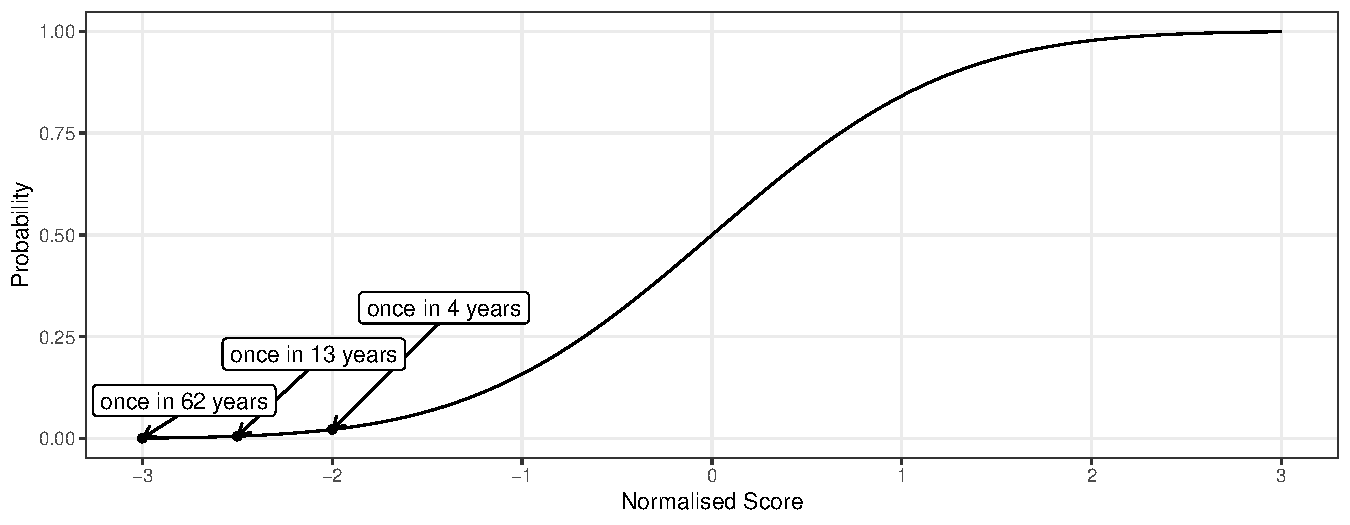
\includegraphics{tidyindex_files/figure-pdf/fig-normalising-1.pdf}

}

\caption{\label{fig-normalising}Scatterplot of normal quantiles against
their density values. THree tail density values are highlighted with its
probability of occurence labelled. Probability is calculated assuming
monthly data: with a density of -2, the probability of occurrence is
1/pnorm(-2)/12 = 4 years. The non-linear relationship between the two
quantities suggests normalised indexes need to be interpreted with
caution since a slight change in the tail distribution can result in
magnitudes of difference in its probability of occurrence.}

\end{figure}

\hypertarget{benchmarking}{%
\subsubsection{Benchmarking}\label{benchmarking}}

Benchmarking sets a constant value to allow the constructed index to be
compared across time. Here we denote it with \(u[x(s_i, t_j)]\) where
\(u\) is a scalar of interest in the index constructed. A benchmark
value could be a constant or a function of the data, i.e.~mean.

\hypertarget{simplification}{%
\subsubsection{Simplification}\label{simplification}}

In public communication, the index values are usually accompanied by a
categorical grade. The categorised grades are an ordered set of
descriptive words or colors to communicate the severity or guide the
comprehension of the indexes. The mapping from continuous index values
to the discrete grades is called simplification in the pipeline and it
can be written as a piece-wise function:

\begin{equation}
\begin{cases}
C_0 & c_1 \leq (s_i; t_j) < c_0 \\
C_1 & c_2 \leq x(s_i; t_j) < c_1 \\
C_2 & c_3 \leq x(s_i; t_j) < c_2 \\
\cdots \\
C_z & c_z \leq x(s_i; t_j)
\end{cases}
\end{equation}

where \(C_0, C_1,\cdots ,C_z\) are the categories and
\(c_0, c_1, \cdots, c_z\) are the thresholds for each category. In SPI,
droughts are sorted into four categories: mild drought: \([-0.99, 0]\);
moderate drought: \([-1.49, -1]\); severe drought: \([-1.99, -1.5]\),
and extreme drought: \([-\infty, -2]\). In this case,
\(C_0, C_1, C_2, C_3\) are the drought categories: mild, moderate,
severe, and extreme drought (\(z = 3\)) and
\(c_0 =0, c_1 = -1, c_2 = -1.5, c_3 = -2\) are the cutoff value for each
class.

\hypertarget{sec-dev}{%
\section{Incorporating alternative methods into the pipeline
components}\label{sec-dev}}

\hypertarget{sec-examples}{%
\section{Examples}\label{sec-examples}}

\hypertarget{a-drought-index-example}{%
\subsection{A drought index example}\label{a-drought-index-example}}

A common task for drought researchers is to compute indexes at different
parameter combinations. This can be used to identify the spatial and
temporal extent of drought events, recommend the best parameter choice,
or compare the effectiveness of indexes for monitoring drought. The
example below computes two indexes: SPI and SPEI, at various time scales
and fitted distributions, for stations in the state of Queensland in
Australia. The purpose of the example is to demonstrate the interfaces
the tidyindex package built to allow easy computing at different
parameter combinations.

The state of Queensland in Australia is frequently affected by natural
disaster events such as flood and drought, which can have significant
impacts on its agricultural industry. This study uses daily data from
Global Historical Climatology Network Daily (GHCND), accessed via the
package \texttt{rnoaa} to examine drought/flood condition in Queensland.
Daily data is average into monthly and stations are excluded if monthly
data contains missings, which is required for calculating both SPI and
SPEI. This gives 29 stations with complete records from 1990 January to
2022 April.

The function \texttt{compute\_indexes()} can be used to collectively
compute multiple indexes. The tidyindex offers wrapper functions, with
the prefix idx\_, that simplify the calculation of commonly used indexes
by combining a set of pipeline steps into a single function. For
example, the function \texttt{idx\_spei()} includes the five steps
previously described in Section~\ref{sec-toy-example} (variable
transformation, dimension reduction, temporal aggregation, distribution
fit, and normalise). Each \texttt{idx\_xxx()} function specifies the
relevant parameters relevant to the index: the thornthwaite method is
used to calculate PET in SPEI, with the average temperature
(\texttt{tavg}) and latitude (\texttt{lat}) used as inputs. The SPEI is
computed at four time scales (6, 12, 24, and 36 months) and fitted with
two distributions (Log-logistic and General Extreme Value (GEV)). The
SPI is also computed at the same four time scales and uses the default
gamma distribution to fit the aggregated series.

\begin{Shaded}
\begin{Highlighting}[]
\NormalTok{.scale }\OtherTok{\textless{}{-}} \FunctionTok{c}\NormalTok{(}\DecValTok{6}\NormalTok{, }\DecValTok{12}\NormalTok{, }\DecValTok{24}\NormalTok{, }\DecValTok{36}\NormalTok{)}
\NormalTok{(idx }\OtherTok{\textless{}{-}}\NormalTok{ queensland }\SpecialCharTok{\%\textgreater{}\%}
  \FunctionTok{init}\NormalTok{(}\AttributeTok{id =}\NormalTok{ id, }\AttributeTok{time =}\NormalTok{ ym) }\SpecialCharTok{\%\textgreater{}\%}
  \FunctionTok{compute\_indexes}\NormalTok{(}
    \AttributeTok{spei =} \FunctionTok{idx\_spei}\NormalTok{(}
      \AttributeTok{.pet\_method =} \StringTok{"thornthwaite"}\NormalTok{, }\AttributeTok{.tavg =}\NormalTok{ tavg, }\AttributeTok{.lat =}\NormalTok{ lat,}
      \AttributeTok{.scale =}\NormalTok{ .scale, }\AttributeTok{.dist =} \FunctionTok{c}\NormalTok{(}\FunctionTok{gev}\NormalTok{(), }\FunctionTok{loglogistic}\NormalTok{())),}
    \AttributeTok{spi =} \FunctionTok{idx\_spi}\NormalTok{(}\AttributeTok{.scale =}\NormalTok{ .scale)}
\NormalTok{  ))}
\end{Highlighting}
\end{Shaded}

\begin{verbatim}
[1] "Checking for missing values (`NA`): all the data must be complete. Input type is vector. Assuming the data are monthly time series starting in January, all regular (non-leap) years."
\end{verbatim}

\begin{verbatim}
# A tibble: 128,586 x 19
   .idx  .period id              ym  prcp  tmax  tmin  tavg  long   lat name    pet   diff
   <chr>   <dbl> <chr>        <mth> <dbl> <dbl> <dbl> <dbl> <dbl> <dbl> <chr> <dbl>  <dbl>
 1 spei        6 ASN00029~ 1990 Jun   170  29.7  16.2  23.0  142. -15.5 KOWA~  85.9   84.1
 2 spei        6 ASN00029~ 1990 Jun   170  29.7  16.2  23.0  142. -15.5 KOWA~  85.9   84.1
 3 spei        6 ASN00029~ 1990 Jun     0  23.0  11.8  17.4  139. -20.7 MOUN~  47.6  -47.6
 4 spei        6 ASN00029~ 1990 Jun     0  23.0  11.8  17.4  139. -20.7 MOUN~  47.6  -47.6
 5 spei        6 ASN00031~ 1990 Jun   794  25.8  18.1  21.9  146. -16.9 CAIR~  80.3  714. 
 6 spei        6 ASN00031~ 1990 Jun   794  25.8  18.1  21.9  146. -16.9 CAIR~  80.3  714. 
 7 spei        6 ASN00031~ 1990 Jun   504  23.0  13.8  18.4  145. -17.1 WALK~  48.0  456. 
 8 spei        6 ASN00031~ 1990 Jun   504  23.0  13.8  18.4  145. -17.1 WALK~  48.0  456. 
 9 spei        6 ASN00032~ 1990 Jun  1970  23.9  16.4  20.2  146. -17.6 SOUT~  70.2 1900. 
10 spei        6 ASN00032~ 1990 Jun  1970  23.9  16.4  20.2  146. -17.6 SOUT~  70.2 1900. 
# i 128,576 more rows
# i 6 more variables: .scale <dbl>, .agg <dbl>, .method <chr>, .fitted <dbl>,
#   .dist <chr>, .index <dbl>
\end{verbatim}

The output from \texttt{compute\_indexes()} contains index values and
associated parameter in a long tibble. It includes the original
variables (\texttt{id}, \texttt{ym}, \texttt{prcp}, \texttt{tmax},
\texttt{tmin}, \texttt{tavg}, \texttt{long}, \texttt{lat}, and
\texttt{name}), index parameters (\texttt{.idx}, \texttt{.scale},
\texttt{.method}, and \texttt{.dist}), intermediate variables
(\texttt{pet}, \texttt{.agg}, and \texttt{.fitted}), and the final index
(\texttt{.index}). This data can be visualised across space or time, or
simultaneously, to explore the wet/dry condition in Queensland.
Figure~\ref{fig-compute-spatial} visualises the spatial distribution of
SPI at two periods (2010 October - 2011 March and 2019 October - 2020
March) with significant natural disaster events: 2010/11 Queensland
flood and 2019 Australia drought, which contributes to the notorious
2019/20 bushfire. Figure~\ref{fig-compute-temporal} displays the
sensitivity of the SPEI series for one particular station, Texas post
office, at different time scales and fitted distributions. These two
plots demonstrate some possibilities to explore the indexes after they
are computed from \texttt{compute\_indexes()}.

\begin{figure}

{\centering 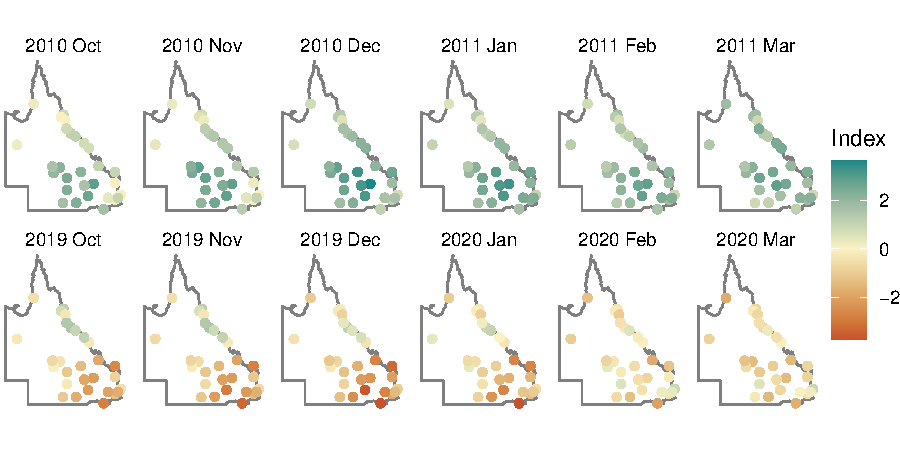
\includegraphics{tidyindex_files/figure-pdf/fig-compute-spatial-1.pdf}

}

\caption{\label{fig-compute-spatial}Spatial distribution of Standardized
Precipitation Index (SPI-12) in Queensland, Australia during two major
flood and drought events: 2010/11 and 2019/20. The map shows a continous
wet period during the 2010/11 flood period and a mitigated drought
situation, after its worst in 2019 December and 2020 Janurary, likely
due to the increased rainfall in February from the meteorological
record.}

\end{figure}

\begin{figure}

{\centering 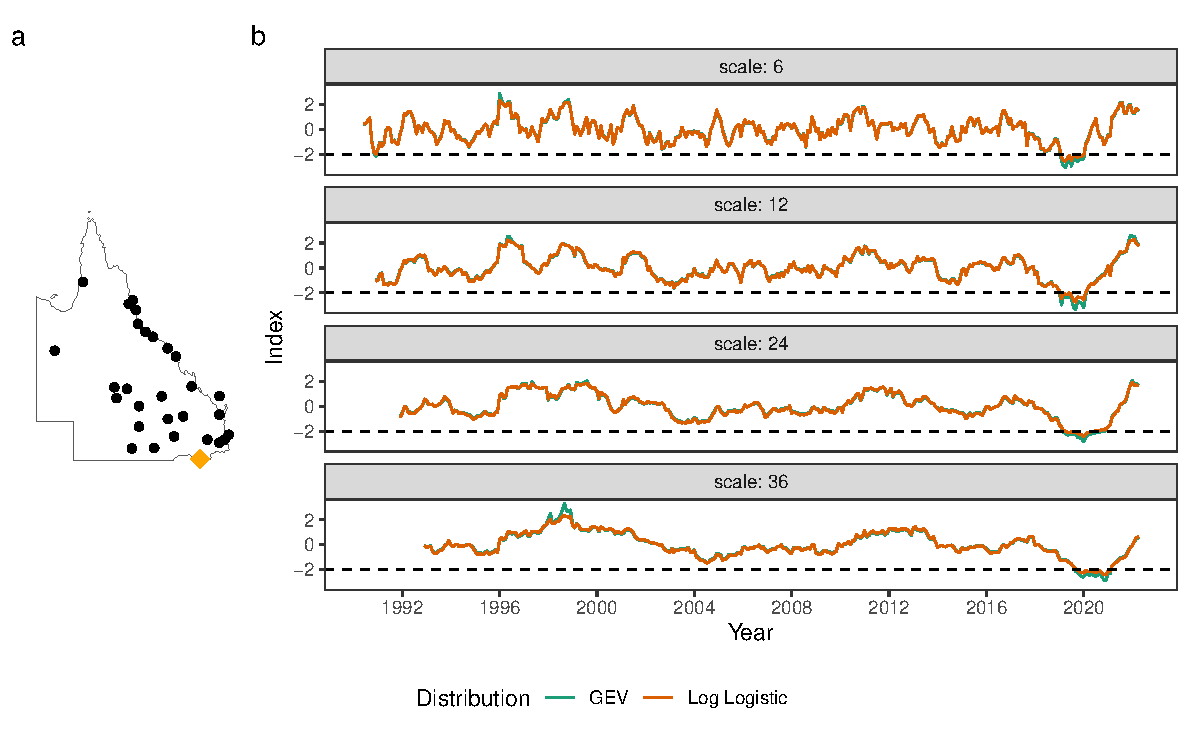
\includegraphics{tidyindex_files/figure-pdf/fig-compute-temporal-1.pdf}

}

\caption{\label{fig-compute-temporal}Time series plot of Standardized
Precipitation-Evapotranspiration Index (SPEI) at the Texas post office
station (highlighted by a diamond shape in panel a). The SPEI is
calculated at four time scales (6, 12, 24, and 36 months) and fitted
with two distributions (Log Logistic and GEV). The dashed line at -2
represents the class ``extreme drought'' by the SPEI. A larger time
scale gives a smoother index series, while also takes longer to recover
from an extreme situation as seen in the 2019/20 drought period. The
SPEI values from two distribution fits mostly agree, while GEV can
results in more extreme values, i.e.~in 1998 and 2020.}

\end{figure}

\hypertarget{an-example-on-sustainable-development-indicators}{%
\subsection{An example on sustainable development
indicators}\label{an-example-on-sustainable-development-indicators}}

In the following example, the Human Development Index (HDI) will first
be constructed using the pipeline syntax. The section will then
demonstrate how expressions or parameters in the pipeline can be swapped
to alternatives to study the index property.

Human Development Index (HDI) measures the development of countries
through more than just economic growth, but also people's life
expectancy and opportunity to receive education. These three identified
dimensions are measured using four indicators: life expectancy at birth
(health), expected years of schooling (education), mean years of
schooling (education), and Gross National Income (GNI) \emph{per capita}
(standard of living). The technical notes (United Nations Development
Programme 2021) have documented the procedures to calculate HDI and they
are summarised below:

\begin{enumerate}
\def\labelenumi{\arabic{enumi}.}
\tightlist
\item
  take log on GNI \emph{per capita},
\item
  rescale the four indicators into {[}0, 1{]} using mini-max,
\item
  aggregate the two education indicators using arithmetic mean, and
\item
  aggregate the three dimensions into the index using geometric mean.
\end{enumerate}

The values used in mini-max rescaling are summarised in
Table~\ref{tbl-rescale-params} and the justification of these numbers
can be found in the technical notes mentioned above.

\hypertarget{tbl-rescale-params}{}
\begin{longtable}[]{@{}
  >{\raggedright\arraybackslash}p{(\columnwidth - 8\tabcolsep) * \real{0.2375}}
  >{\raggedright\arraybackslash}p{(\columnwidth - 8\tabcolsep) * \real{0.4500}}
  >{\raggedright\arraybackslash}p{(\columnwidth - 8\tabcolsep) * \real{0.1125}}
  >{\raggedleft\arraybackslash}p{(\columnwidth - 8\tabcolsep) * \real{0.1000}}
  >{\raggedleft\arraybackslash}p{(\columnwidth - 8\tabcolsep) * \real{0.1000}}@{}}
\caption{\label{tbl-rescale-params}Maximum and minimum values used to
rescale the four HDI indicators into {[}0, 1{]} range. The maximum of
GNI per capita is taken as the common log of 75,000, approximatly
4.875.}\tabularnewline
\toprule()
\begin{minipage}[b]{\linewidth}\raggedright
Dimension
\end{minipage} & \begin{minipage}[b]{\linewidth}\raggedright
Indicator
\end{minipage} & \begin{minipage}[b]{\linewidth}\raggedright
Variable
\end{minipage} & \begin{minipage}[b]{\linewidth}\raggedleft
Minimum
\end{minipage} & \begin{minipage}[b]{\linewidth}\raggedleft
Maximum
\end{minipage} \\
\midrule()
\endfirsthead
\toprule()
\begin{minipage}[b]{\linewidth}\raggedright
Dimension
\end{minipage} & \begin{minipage}[b]{\linewidth}\raggedright
Indicator
\end{minipage} & \begin{minipage}[b]{\linewidth}\raggedright
Variable
\end{minipage} & \begin{minipage}[b]{\linewidth}\raggedleft
Minimum
\end{minipage} & \begin{minipage}[b]{\linewidth}\raggedleft
Maximum
\end{minipage} \\
\midrule()
\endhead
Health & Life expectancy at birth (years) & life\_exp & 20 & 85.000 \\
Education & Expected years of schooling (years) & exp\_sch & 0 &
18.000 \\
Education & Mean years of schooling (years) & avg\_sch & 0 & 15.000 \\
Standard of living & GNI per capita (2017 PPP\$) & gni\_pc & 2 &
4.875 \\
\bottomrule()
\end{longtable}

Among the four steps listed in the calculation, the first two are
variable transformation. The next two can be considered as the dimension
reduction step in the data pipeline given its intention to combine
multivariate data into univariate. With the index pipeline proposed in
the paper, HDI can be calculated as:

\begin{Shaded}
\begin{Highlighting}[]
\NormalTok{dt }\OtherTok{\textless{}{-}}\NormalTok{ raw }\SpecialCharTok{\%\textgreater{}\%} \FunctionTok{init}\NormalTok{(}\AttributeTok{id =}\NormalTok{ country, }\AttributeTok{indicators =}\NormalTok{ life\_exp}\SpecialCharTok{:}\NormalTok{gni\_pc)}
\NormalTok{res }\OtherTok{\textless{}{-}}\NormalTok{ dt }\SpecialCharTok{\%\textgreater{}\%}
  \FunctionTok{var\_trans}\NormalTok{(}\AttributeTok{gni\_pc =} \FunctionTok{log}\NormalTok{(gni\_pc, }\AttributeTok{base =} \DecValTok{10}\NormalTok{)) }\SpecialCharTok{\%\textgreater{}\%} 
  \FunctionTok{var\_trans}\NormalTok{(}\AttributeTok{.method =}\NormalTok{ rescale\_minmax, }\AttributeTok{.vars =}\NormalTok{ life\_exp}\SpecialCharTok{:}\NormalTok{gni\_pc,}
            \AttributeTok{min =} \FunctionTok{c}\NormalTok{(}\DecValTok{20}\NormalTok{, }\DecValTok{0}\NormalTok{, }\DecValTok{0}\NormalTok{, }\DecValTok{2}\NormalTok{), }\AttributeTok{max =} \FunctionTok{c}\NormalTok{(}\DecValTok{85}\NormalTok{, }\DecValTok{18}\NormalTok{, }\DecValTok{15}\NormalTok{, }\FunctionTok{log10}\NormalTok{(}\DecValTok{75000}\NormalTok{))) }\SpecialCharTok{\%\textgreater{}\%} 
  \FunctionTok{dim\_red}\NormalTok{(}\AttributeTok{sch =}\NormalTok{ (exp\_sch }\SpecialCharTok{+}\NormalTok{ avg\_sch) }\SpecialCharTok{/} \DecValTok{2}\NormalTok{) }\SpecialCharTok{\%\textgreater{}\%}
  \FunctionTok{dim\_red}\NormalTok{(}\AttributeTok{index =}\NormalTok{ (life\_exp }\SpecialCharTok{*}\NormalTok{ sch }\SpecialCharTok{*}\NormalTok{ gni\_pc)}\SpecialCharTok{\^{}}\NormalTok{(}\DecValTok{1}\SpecialCharTok{/}\DecValTok{3}\NormalTok{))}
\end{Highlighting}
\end{Shaded}

Index analysts can be interested in studying the property of the index
and the countries through the ``what-if'' questions. In the context of
HDI, this can be what if an alternative dimension reduction expression
is used to reduce the three dimensions into the HDI? Apart from the
geometrical mean, linear combination is a common method to reduce the
data dimension. With different weighting schemes, the combination can be
compared to study the variable importance of each dimension or to reveal
the underlying structures of countries. The following code tests five
expressions (arithmetic mean, principal component analysis weight, and
three weighting schemes emphasizing life expectancy, education, and GNI
per capita respectively) using the \texttt{swap\_exprs()} function. The
function first locates the operation to be tested
(\texttt{.var\ =\ index}), then accepts a list of expressions for
testing \texttt{.expr}, before requesting the raw data:

\begin{Shaded}
\begin{Highlighting}[]
\NormalTok{(res2 }\OtherTok{\textless{}{-}}\NormalTok{ res }\SpecialCharTok{\%\textgreater{}\%}
  \FunctionTok{swap\_exprs}\NormalTok{(}
    \AttributeTok{.var =}\NormalTok{ index,}
    \AttributeTok{.expr =} \FunctionTok{list}\NormalTok{(}
      \AttributeTok{index1 =}\NormalTok{ (life\_exp }\SpecialCharTok{+}\NormalTok{ sch }\SpecialCharTok{+}\NormalTok{ gni\_pc)}\SpecialCharTok{/}\DecValTok{3}\NormalTok{,}
      \CommentTok{\# PCA recommended weight}
      \AttributeTok{index2 =} \FloatTok{0.569} \SpecialCharTok{*}\NormalTok{ life\_exp }\SpecialCharTok{+} \FloatTok{0.576} \SpecialCharTok{*}\NormalTok{ sch }\SpecialCharTok{+} \FloatTok{0.586} \SpecialCharTok{*}\NormalTok{ gni\_pc, }
      \AttributeTok{index3 =} \FloatTok{0.8} \SpecialCharTok{*}\NormalTok{ life\_exp }\SpecialCharTok{+} \FloatTok{0.1} \SpecialCharTok{*}\NormalTok{ sch }\SpecialCharTok{+} \FloatTok{0.1} \SpecialCharTok{*}\NormalTok{ gni\_pc,}
      \AttributeTok{index4 =} \FloatTok{0.1} \SpecialCharTok{*}\NormalTok{ life\_exp }\SpecialCharTok{+} \FloatTok{0.8} \SpecialCharTok{*}\NormalTok{ sch }\SpecialCharTok{+} \FloatTok{0.1} \SpecialCharTok{*}\NormalTok{ gni\_pc,}
      \AttributeTok{index5 =} \FloatTok{0.1} \SpecialCharTok{*}\NormalTok{ life\_exp }\SpecialCharTok{+} \FloatTok{0.1} \SpecialCharTok{*}\NormalTok{ sch }\SpecialCharTok{+} \FloatTok{0.8} \SpecialCharTok{*}\NormalTok{ gni\_pc),}
    \AttributeTok{.raw\_data =}\NormalTok{ dt))}
\end{Highlighting}
\end{Shaded}

\begin{verbatim}
Index pipeline: 

Summary: 
\end{verbatim}

\begin{verbatim}
var_trans: `log(gni_pc, base = 10)` -> gni_pc
\end{verbatim}

\begin{verbatim}
var_trans: `rescale_minmax(var = life_exp, min = 20, max = 85)` ->
life_exp
\end{verbatim}

\begin{verbatim}
var_trans: `rescale_minmax(var = exp_sch, min = 0, max = 18)` ->
exp_sch
\end{verbatim}

\begin{verbatim}
var_trans: `rescale_minmax(var = avg_sch, min = 0, max = 15)` ->
avg_sch
\end{verbatim}

\begin{verbatim}
var_trans: `rescale_minmax(var = gni_pc, min = 2, max = 4.875061)` ->
gni_pc
\end{verbatim}

\begin{verbatim}
dim_red: `(exp_sch + avg_sch)/2` -> sch
\end{verbatim}

\begin{verbatim}
dim_red: `(life_exp * sch * gni_pc)^(1/3)` -> index0
\end{verbatim}

\begin{verbatim}
dim_red: `(life_exp + sch + gni_pc)/3` -> index1
\end{verbatim}

\begin{verbatim}
dim_red: `0.569 * life_exp + 0.576 * sch + 0.586 * gni_pc` -> index2
\end{verbatim}

\begin{verbatim}
dim_red: `0.8 * life_exp + 0.1 * sch + 0.1 * gni_pc` -> index3
\end{verbatim}

\begin{verbatim}
dim_red: `0.1 * life_exp + 0.8 * sch + 0.1 * gni_pc` -> index4
\end{verbatim}

\begin{verbatim}
dim_red: `0.1 * life_exp + 0.1 * sch + 0.8 * gni_pc` -> index5
\end{verbatim}

\begin{verbatim}

Data: 
# A tibble: 191 x 13
      id country   life_exp exp_sch avg_sch gni_pc   sch index0 index1
   <dbl> <chr>        <dbl>   <dbl>   <dbl>  <dbl> <dbl>  <dbl>  <dbl>
 1     1 Switzerl~    0.984   0.917   0.924  0.983 0.920  0.962  0.963
 2     2 Norway       0.973   1       0.867  0.978 0.933  0.961  0.961
 3     3 Iceland      0.964   1       0.918  0.955 0.959  0.959  0.959
 4     4 Hong Kon~    1       0.960   0.815  0.973 0.887  0.952  0.953
 5     5 Australia    0.993   1       0.848  0.936 0.924  0.951  0.951
 6     6 Denmark      0.944   1       0.864  0.967 0.932  0.948  0.948
 7     7 Sweden       0.969   1       0.841  0.952 0.920  0.947  0.947
 8     8 Ireland      0.954   1       0.772  1     0.886  0.945  0.947
 9     9 Germany      0.933   0.945   0.939  0.952 0.942  0.942  0.942
10    10 Netherla~    0.949   1       0.839  0.956 0.919  0.941  0.941
# i 181 more rows
# i 4 more variables: index2 <dbl>, index3 <dbl>, index4 <dbl>,
#   index5 <dbl>
\end{verbatim}

The resulting data includes five more columns corresponding to the five
alternative indexes. The country ranking can be further computed on the
data and plotted in a scatterplot matrix as in
Figure~\ref{fig-hdi-expr}. The plot shows almost similar ranks suggested
by the indexes calculated using geometric mean (\texttt{rank0}), the
arithmetic mean (\texttt{rank1}), and the PCA recommended weights
(\texttt{rank2}). The agreement of the three methods supports the use of
geometric mean as the dimension reduction method in the original index.
The scatterplot matrix also reveals the difference in ranking when the
three dimensions are given different weights in \texttt{rank3},
\texttt{rank4}, and \texttt{rank5}. The panel \texttt{rank4} vs
\texttt{rank5} shows a cluster of highlighted points with relatively
high ranks according to \texttt{rank5} but low in \texttt{rank4}. These
countries are printed in Table~\ref{tbl-hdi-expr} prints along with
their three dimensions, calculated indexes, and rankings. While having a
high life expectancy and GNI \emph{per capita}, these countries
(Andorra, Qatar, San Marino, Kuwait, and Brunei Darussalam) score
relatively low in education, which is weighted heavily in
\texttt{index4}
(\texttt{0.1\ *\ life\_exp\ +\ 0.1\ *\ sch\ +\ 0.8\ *\ gni\_pc}).

\begin{figure}

{\centering 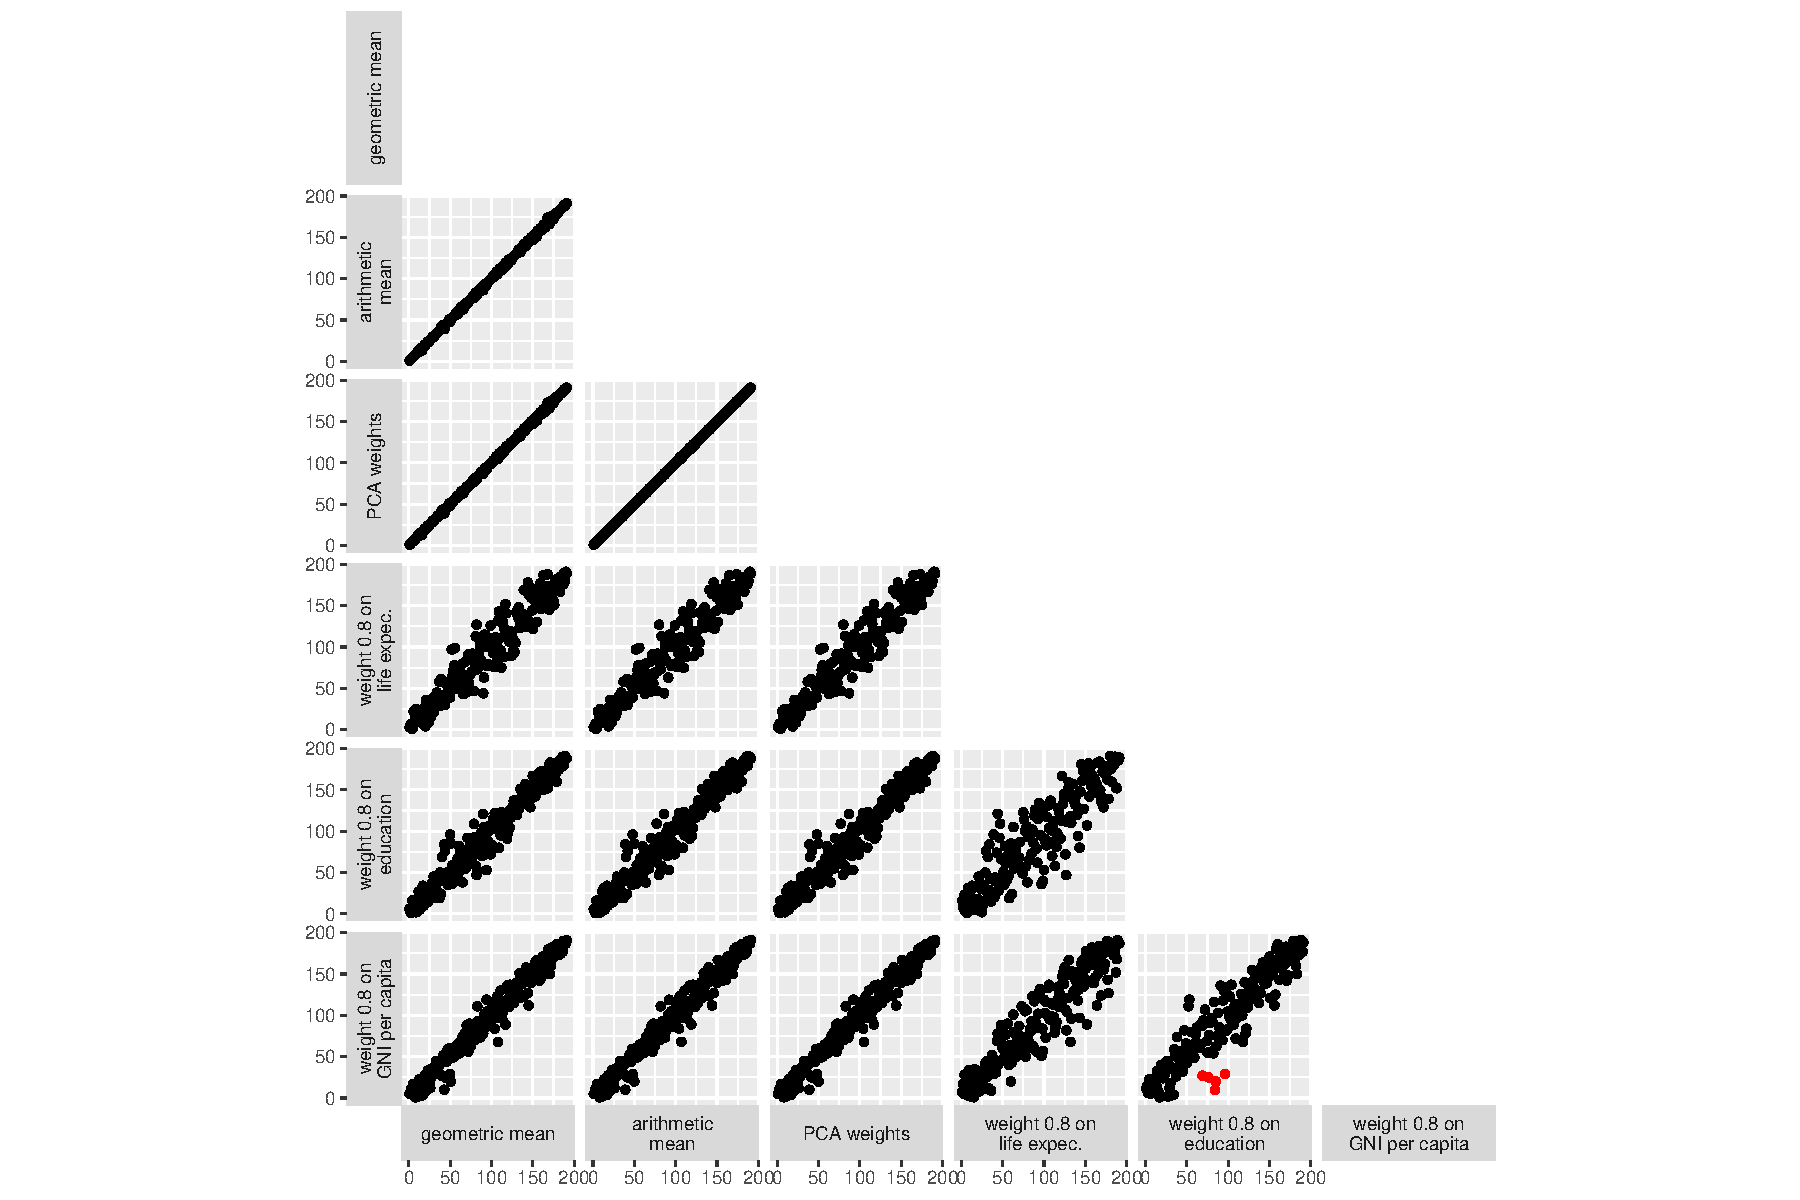
\includegraphics{tidyindex_files/figure-pdf/fig-hdi-expr-1.pdf}

}

\caption{\label{fig-hdi-expr}Comparing country ranks from six different
index constructions: geometric mean (\texttt{rank0}), arithmetic mean
(\texttt{rank1}), principal component analysis recommended weights
(\texttt{rank2}), and heavier weight on life expectancy, education, and
GNI per capita (\texttt{rank3} - \texttt{rank5}). Geometric mean,
arithmetic mean, and PCA produce similar rankings where countries are
aligned in a diagnoal line, while country rankings varies when compare
among \texttt{rank3} to \texttt{rank5}. Panel \texttt{rank5}
vs.~\texttt{rank4} highlights a cluster of countries that rank high by
\texttt{rank5} but low by \texttt{rank4}. The plot demonstrates the
necessity to test on various alternative expressions to verify the
robustness of the method and to capture distinctive characteristics of
different countries.}

\end{figure}

\hypertarget{tbl-hdi-expr}{}
\begin{longtable}[]{@{}
  >{\raggedright\arraybackslash}p{(\columnwidth - 14\tabcolsep) * \real{0.2118}}
  >{\raggedleft\arraybackslash}p{(\columnwidth - 14\tabcolsep) * \real{0.1882}}
  >{\raggedleft\arraybackslash}p{(\columnwidth - 14\tabcolsep) * \real{0.1176}}
  >{\raggedleft\arraybackslash}p{(\columnwidth - 14\tabcolsep) * \real{0.1765}}
  >{\raggedleft\arraybackslash}p{(\columnwidth - 14\tabcolsep) * \real{0.0824}}
  >{\raggedleft\arraybackslash}p{(\columnwidth - 14\tabcolsep) * \real{0.0824}}
  >{\raggedleft\arraybackslash}p{(\columnwidth - 14\tabcolsep) * \real{0.0706}}
  >{\raggedleft\arraybackslash}p{(\columnwidth - 14\tabcolsep) * \real{0.0706}}@{}}
\caption{\label{tbl-hdi-expr}A selected number of countries with low
rankings when education is given a heavy weight (\texttt{index4}) while
ranks high when a heavier weight is given on GNI per capital
(\texttt{index5}).}\tabularnewline
\toprule()
\begin{minipage}[b]{\linewidth}\raggedright
country
\end{minipage} & \begin{minipage}[b]{\linewidth}\raggedleft
life expectancy
\end{minipage} & \begin{minipage}[b]{\linewidth}\raggedleft
education
\end{minipage} & \begin{minipage}[b]{\linewidth}\raggedleft
GNI per capita
\end{minipage} & \begin{minipage}[b]{\linewidth}\raggedleft
index3
\end{minipage} & \begin{minipage}[b]{\linewidth}\raggedleft
index4
\end{minipage} & \begin{minipage}[b]{\linewidth}\raggedleft
rank3
\end{minipage} & \begin{minipage}[b]{\linewidth}\raggedleft
rank4
\end{minipage} \\
\midrule()
\endfirsthead
\toprule()
\begin{minipage}[b]{\linewidth}\raggedright
country
\end{minipage} & \begin{minipage}[b]{\linewidth}\raggedleft
life expectancy
\end{minipage} & \begin{minipage}[b]{\linewidth}\raggedleft
education
\end{minipage} & \begin{minipage}[b]{\linewidth}\raggedleft
GNI per capita
\end{minipage} & \begin{minipage}[b]{\linewidth}\raggedleft
index3
\end{minipage} & \begin{minipage}[b]{\linewidth}\raggedleft
index4
\end{minipage} & \begin{minipage}[b]{\linewidth}\raggedleft
rank3
\end{minipage} & \begin{minipage}[b]{\linewidth}\raggedleft
rank4
\end{minipage} \\
\midrule()
\endhead
Andorra & 0.929 & 0.721 & 0.942 & 0.909 & 0.764 & 32 & 69 \\
Qatar & 0.912 & 0.684 & 1.000 & 0.898 & 0.739 & 34 & 84 \\
San Marino & 0.937 & 0.701 & 0.947 & 0.914 & 0.749 & 30 & 76 \\
Kuwait & 0.903 & 0.670 & 0.947 & 0.884 & 0.721 & 39 & 96 \\
Brunei Darussalam & 0.841 & 0.694 & 0.977 & 0.840 & 0.737 & 60 & 85 \\
\bottomrule()
\end{longtable}

\newpage

\hypertarget{conclusion}{%
\section{Conclusion}\label{conclusion}}

The paper presents a data pipeline with nine modules for constructing
and analysing indexes. The pipeline increases transparency in the
practice for index analysts to experiment with different index design
and parameter choices to better design and apply their indexes. The
significance of this work is its ability to provide a universal
framework for index construction, which can be applied across different
domains.

Examples have been given in the drought indexes and human development
index to demonstrate computing of indexes with different parameters
combinations and how alternative index design can provide insights to
understand distinctive country characteristics that could sometimes be
overlooked. The accompanied package, tidyindex, is not meant to provide
comprehensive implementation for all indexes across all domains.
Instead, it demonstrates implementing individual pipeline steps that are
versatile to multiple indexes and composing new indexes from existing
steps. Domain experts are welcomed to adopt the pipeline approach to
develop specialised packages for specific-domains indexes.

\hypertarget{reference}{%
\section*{Reference}\label{reference}}
\addcontentsline{toc}{section}{Reference}

\hypertarget{refs}{}
\begin{CSLReferences}{1}{0}
\leavevmode\vadjust pre{\hypertarget{ref-buja_elements_1988}{}}%
Buja, A, D Asimov, C Hurley, and JA McDonald. 1988. {``Elements of a
Viewing Pipeline for Data Analysis.''} In \emph{Dynamic Graphics for
Statistics}, 277--308. Wadsworth, Belmont.

\leavevmode\vadjust pre{\hypertarget{ref-oecd_handbook_2008}{}}%
OECD, European Union, and Joint Research Centre - European Commission.
2008. \emph{Handbook on {Constructing} {Composite} {Indicators}:
{Methodology} and {User} {Guide}}. OECD.
\url{https://doi.org/10.1787/9789264043466-en}.

\leavevmode\vadjust pre{\hypertarget{ref-sutherland_orca_2000}{}}%
Sutherland, Peter, Anthony Rossini, Thomas Lumley, Nicholas Lewin-Koh,
Julie Dickerson, Zach Cox, and Dianne Cook. 2000. {``Orca: {A}
{Visualization} {Toolkit} for {High}-{Dimensional} {Data}.''}
\emph{Journal of Computational and Graphical Statistics} 9 (3): 509--29.
\url{https://www.jstor.org/stable/1390943}.

\leavevmode\vadjust pre{\hypertarget{ref-tucker_red_1979}{}}%
Tucker, Compton J. 1979. {``Red and Photographic Infrared Linear
Combinations for Monitoring Vegetation.''} \emph{Remote Sensing of
Environment} 8 (2): 127--50.
\url{https://doi.org/10.1016/0034-4257(79)90013-0}.

\leavevmode\vadjust pre{\hypertarget{ref-UNDP_2021_tech_notes}{}}%
United Nations Development Programme. 2021. {``Human Development Report
2021-2022: The Next Frontier: Human Development and the Anthropocene.''}
\url{https://hdr.undp.org/sites/default/files/2021-22_HDR/hdr2021-22_technical_notes.pdf}.

\leavevmode\vadjust pre{\hypertarget{ref-spei}{}}%
Vicente-Serrano, Sergio M., Santiago Beguería, and Juan I. López-Moreno.
2010. {``A {Multiscalar} {Drought} {Index} {Sensitive} to {Global}
{Warming}: {The} {Standardized} {Precipitation} {Evapotranspiration}
{Index}.''} \emph{Journal of Climate} 23 (7): 1696--1718.
\url{https://journals.ametsoc.org/view/journals/clim/23/7/2009jcli2909.1.xml}.

\leavevmode\vadjust pre{\hypertarget{ref-wickham_tidy_2014}{}}%
Wickham, Hadley. 2014. {``Tidy {Data}.''} \emph{Journal of Statistical
Software} 59 (September): 1--23.
\url{https://doi.org/10.18637/jss.v059.i10}.

\leavevmode\vadjust pre{\hypertarget{ref-wickham_plumbing_2009}{}}%
Wickham, Hadley, Michael Lawrence, Dianne Cook, Andreas Buja, Heike
Hofmann, and Deborah F. Swayne. 2009. {``The Plumbing of Interactive
Graphics.''} \emph{Computational Statistics} 24 (2): 207--15.
\url{https://doi.org/10.1007/s00180-008-0116-x}.

\leavevmode\vadjust pre{\hypertarget{ref-xie_reactive_2014}{}}%
Xie, Yihui, Heike Hofmann, and Xiaoyue Cheng. 2014. {``Reactive
{Programming} for {Interactive} {Graphics}.''} \emph{Statistical
Science} 29 (2): 201--13.
\url{https://www.jstor.org/stable/43288470?seq=1}.

\leavevmode\vadjust pre{\hypertarget{ref-climate-indexes}{}}%
Zhang, Xuebin. 2020. {``ETCCDI Climate Change Indices.''}
\url{http://etccdi.pacificclimate.org/index.shtml}.

\end{CSLReferences}



\end{document}
